%!TEX root = booklet.tex

\section{SIGMOD Reception -- Van Gogh Museum (sponsored by MonetDB)}

\vspace{-2mm}

\begin{figure*}[h]
\centering
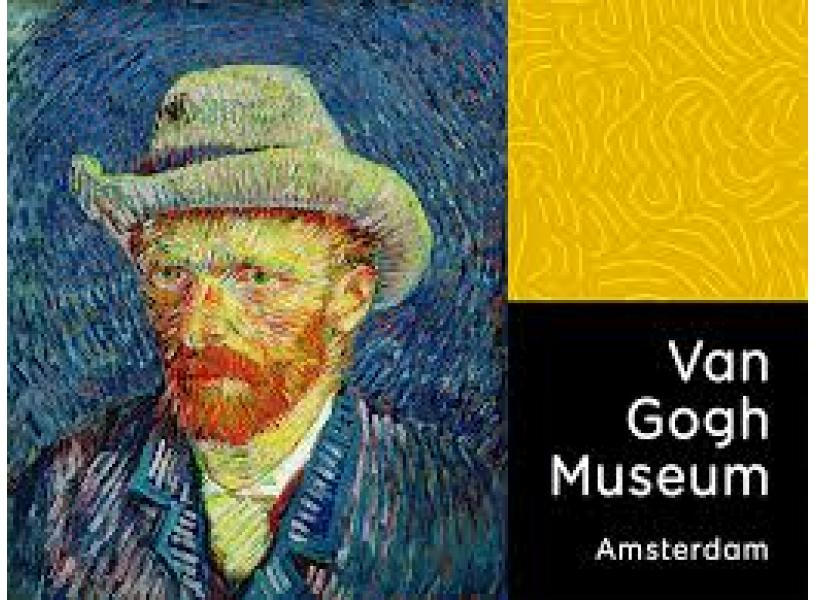
\includegraphics[width=.6\textwidth]{images/reception/vangogh.jpeg}
\end{figure*}


The Van Gogh Museum maintains the world's largest collection of the works of the world's most popular artist - Vincent van Gogh (1853-1890), his paintings, drawings and letters, completed with the art of his contemporaries. Each year, it receives 1.6 million visitors, making it one of the 25 most popular museums in the world.

SIGMOD/PODS'2019 and the event's sponsor \textbf{MonetDB}, are proud to offer all participants registered to the main conference exclusive access to the Van Gogh Museum for the SIGMOD reception on Tuesday July 2, 2019, from 20:30 until 23:00.
Your badge is your ticket into the museum, \textbf{you must bring it with you!}

% 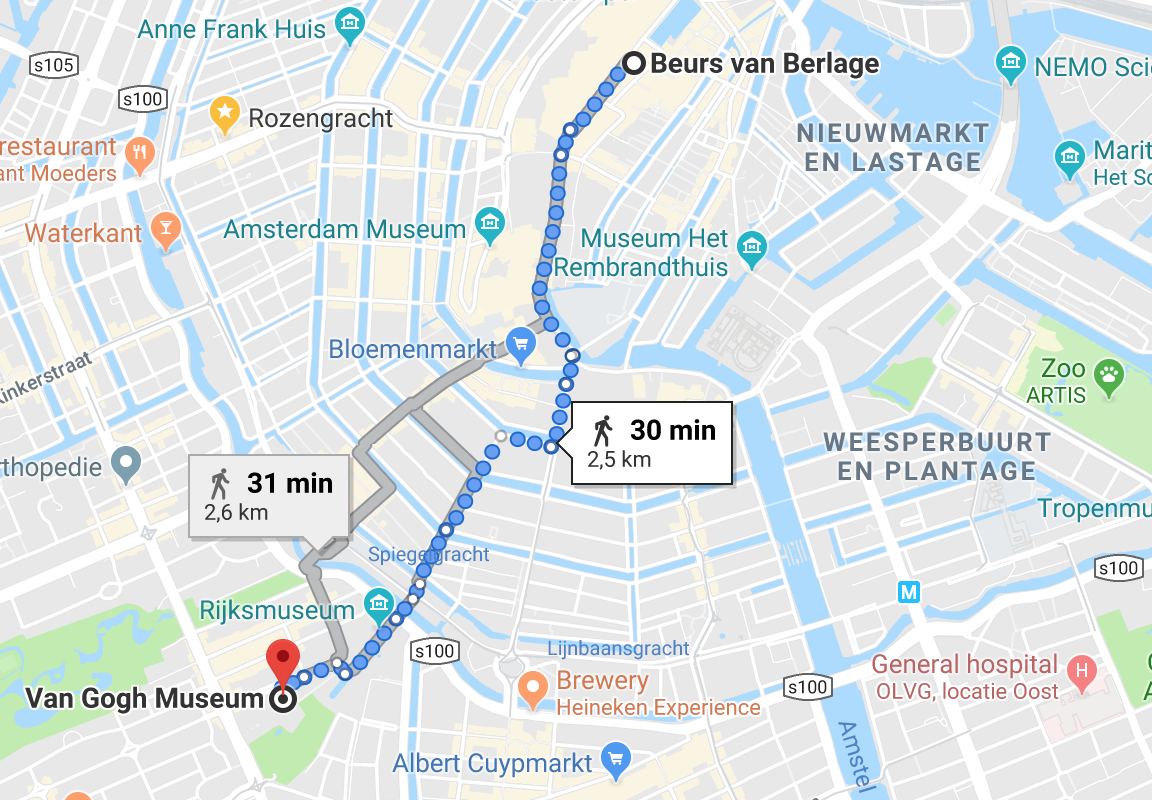
\includegraphics[width=.5\textwidth]{images/reception/berlage-vangogh.png}

There will be time to visit the museum; at the end of the walking route, back in the foyer, there will be drinks and snacks served. The reception food is intended to be dinner-replacing under moderate appetite.

Please note, again, the SIGMOD reception is on \textbf{Tuesday} evening (not Monday evening as usual in SIGMOD). That day, the main program ends around 19:50; so participants have 40 minutes to get to the Museum, which is in the south center of Amsterdam (whereas the Beurs van Berlage conference center is in the middle of the center). You can find the directions in the next page.


\clearpage

\begin{itemize}

\item {Walking}: \hfill 29 min (Instructions: \url{tiny.cc/m3kf7y})

\begin{minipage}{.9\textwidth}
\begin{wrapfigure}[6]{l}{1.9cm}
\vspace*{-1.25\baselineskip}%
\includegraphics[width=1.9cm]{images/reception/vangogh-walking.eps}
\end{wrapfigure}
Leave the venue taking a left and walk south to Dam square, and straight on into Rokin. Continue walking on Rokin until its end, at Munt tower. Continue into Muntplein which becomes Vijzelstraat until crossing the first main canal bridge, after which you take a right onto Herengracht. At the first opportunity you then go left into the Nieuwe Spiegelgracht. Continue this one straight, crossing no less than 4 canals (Prinsen, Keizers, Lijnbaans, Singel). The road passes under the Rijksmuseum; and continuing straight you will hit the Van Gogh museum.
\end{minipage}

\item {Cycling}: \hfill 10 min (Instructions: \url{tiny.cc/m3kf7y})

\begin{minipage}{.9\textwidth}
\begin{wrapfigure}[6]{l}{1.9cm}
\vspace*{-1.25\baselineskip}%
\includegraphics[width=1.9cm]{images/reception/vangogh-walking.eps}
\end{wrapfigure}
You can follow the same route as with walking, above. Use the bicycle path (or street), though, rather than the pedestrian sidewalk.
\vspace{3\baselineskip}
\end{minipage}

\item {Metro 52}: \hfill 19 min (Instructions: \url{tiny.cc/vmkf7y})

\begin{minipage}{.9\textwidth}
\begin{wrapfigure}[6]{l}{1.9cm}
\vspace*{-1.25\baselineskip}%
\includegraphics[width=1.9cm]{images/reception/vangogh-metro.eps}
\end{wrapfigure}
Leave the venue taking a left and walk south to Dam square, and straight on into Rokin. Earlier than indicated on the Google map, right after leaving Dam Square, there is a metro entrance, in front of Hudon's Bay. Metro 52 is Amsterdam's newest metro and its stations are quite beautiful. Take the metro in southward direction (Station Zuid) and exit at the very first stop (Vijzelgracht). Outside, take a right at the big roundabout into Weteringsschans. At the first main crossing, take a left onto the Museumbrug (bridge). The road passes under the Rijksmuseum; and continuing straight you will hit the Van Gogh museum.
~\hspace*{\fill}\mbox{\emph{(Involves ca.\ 16 min walking.)}}
\end{minipage}

\clearpage

\item {Tram 24}: \hfill 20 min (Instructions: \url{tiny.cc/vm6i7y})

\begin{minipage}{.9\textwidth}
\begin{wrapfigure}[6]{l}{1.9cm}
\vspace*{-1.25\baselineskip}%

\includegraphics[width=1.9cm]{images/reception/vangogh-tram-24.png}
\end{wrapfigure}
Leave the venue taking a left and walk south to Dam square. At the tram stop just before Dam square, take tram 24 in southward direction (VU medisch centrum). At the 4th stop (Marie Heinekenplein), just after passing the former Heineken Brewery building (now hosting the "Heineken Experience") leave the tram, walk a few steps back and turn left (westward) into Eerste Jacob van Campenstraat. Continue staight on westward, crossing a canal, until Museum Plein (Square) opens in front of you. On your left-hand side, across the grass field, you see the new entrance hall of the Van Gogh Museum.
~\hspace*{\fill}\mbox{\emph{(Involves ca.\ 12 min walking.)}}
\end{minipage}

\item {Tram 2/12}: \hfill 17 min (Instructions: \url{tiny.cc/fdkf7y})

\begin{minipage}{.9\textwidth}
\begin{wrapfigure}[6]{l}{1.9cm}
\vspace*{-1.25\baselineskip}%
\includegraphics[width=1.9cm]{images/reception/vangogh-tram.eps}
\end{wrapfigure}
Leave the venue taking a left and walk south to Dam square. At Dam square, go right and walk in between the Palace and the Church to the Nieuwezijds Voorburgwal. There is a tram stop there, where you can either take tram 2 or 12  -- they take the same route up until its 7th stop, Van Baerlestraat, where you exit. The tram will just have passed the Van Gogh museum (it is on the left side seen from the tram), so you have to walk back a bit and cross the street.
~\hspace*{\fill}\mbox{\emph{(Involves ca.\ 6 min walking.)}}
\end{minipage}

\end{itemize}


You can of course also try to take a taxi or Uber, but taxi drivers will not be enthusiastically accepting such short trips; doing so will also not be much faster than the other options (or even slower, when stuck in a traffic jam) and quite expensive. Using a car is only recommended if walking is impossible for you. If you just want to minimize walking distance, the last option above (Tram 2 or 12) involves least walking.

\clearpage

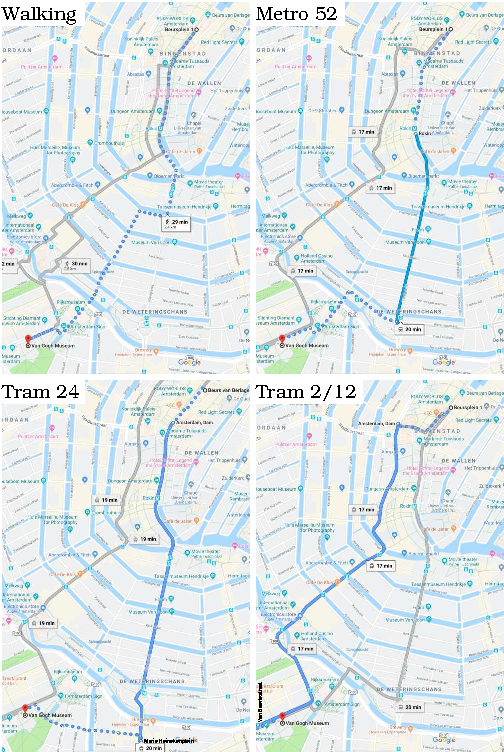
\includegraphics[width=\textwidth]{images/reception/berlage-vangogh-plans.pdf}%
